\section{Simulation results}
\begin{frame}
		\frametitle{Example of identifying $G_1(s)$ in Simulink }
	\begin{itemize}
			\item The simple power system presented was implemented in Simulink.
			\begin{figure}
					\includegraphics[width=0.8\textwidth]{./pictures/G0_sim.tikz}
			\end{figure}
	\end{itemize}
\end{frame}
\begin{frame}
	\frametitle{The identification experiment in the draft requirements}
	\begin{itemize}[<+->]
			\item In the draft requirements they require the power plant owners to replace the input to the governor with their own signal.
			\item They then identify the transfer function from the input to the governor to the electrical power of the generator.
			\begin{equation}\label{eq:G_req}
				G_{req}(s) = -\frac{G_p(s)G_J(s)T(s)}{1+G_J(s)T(s)}
			\end{equation}
			\item This is not $G_p(s)$
	\end{itemize}
\end{frame}
\begin{frame}
		\frametitle{Example of identifying $G_{req}(s)$ in Simulink }
	\begin{itemize}
			\item The transfer function specified in the draft requirements were also estimated in the simulations.
			\begin{figure}
					\includegraphics[width=0.8\textwidth]{./pictures/G_req_sim.tikz}
			\end{figure}
	\end{itemize}
\end{frame}
\begin{frame}
	\frametitle{Estimating the swing dynamics of a power plant}
	\begin{itemize}[<+->]
		\item To find $S(s)$ we need an estimate of $G_J(s)$.
		\item 
			\begin{equation}
				H\approx \frac{\Omega_2 - \Omega_1}{2\Omega_1\Omega_2(|G_1(j\Omega_1)|-|G_1(j\Omega_2)|)}
			\end{equation}
	\end{itemize}
	\begin{equation}\label{eq:S_ident}
		S(s) \approx 2HsG_1(s)
	\end{equation}
	\begin{figure}
		\includegraphics[width=0.8\textwidth]{./pictures/transf_comp.tikz}
	\end{figure}
\end{frame}
\begin{frame}
	\frametitle{Comparison of estimated sensitivity functions}
	\begin{equation}\label{eq:G_sys}
		G_{sys}(s) = \frac{600MW}{0.1Hz}\frac{f_0}{S_{sys}}\frac{1}{2H_{sys}s+K_{d_{sys}}*f_0}
\end{equation}
	\begin{figure}
		\includegraphics[width=0.8\textwidth]{./pictures/S_sim.tikz}
	\end{figure}
\end{frame}
\begin{frame}
		\frametitle{Comparison of estimated $G_1(s)$}
	\begin{equation}\label{eq:G_sys}
		G_{sys}(s) = \frac{600MW}{0.1Hz}\frac{f_0}{S_{sys}}\frac{1}{2H_{sys}s+K_{d_{sys}}*f_0}
\end{equation}
	\begin{figure}
		\includegraphics[width=0.8\textwidth]{./pictures/G0_req_sim.tikz}
	\end{figure}
\end{frame}

\section{Results from a real power plant}
\begin{frame}
	\frametitle{Single line diagram of the plant}
	\begin{figure}
			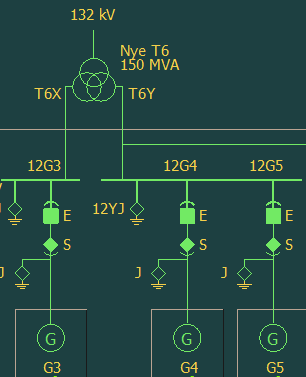
\includegraphics[width=0.8\textwidth]{./pictures/plant.png}
	\end{figure}
\end{frame}
\begin{frame}
	\frametitle{Datasets used}
	\begin{figure}
			\includegraphics[width=0.8\textwidth]{./pictures/signals.tikz}
	\end{figure}
\end{frame}
\begin{frame}
		\frametitle{Identified $G_1(s)$ using pmu signals}
	\begin{figure}
			\includegraphics[width=0.8\textwidth]{./pictures/lyon.tikz}
	\end{figure}
\end{frame}
\begin{frame}
		\frametitle{Identified $G_{req}(s)$ using control system signals}
	\begin{figure}
			\includegraphics[width=0.8\textwidth]{./pictures/req_vs_pmu.tikz}
	\end{figure}
\end{frame}
\begin{frame}
	\frametitle{Estimated sensitivity functions}
		\begin{figure}[tb]
			\includegraphics[width=0.8\textwidth]{./pictures/S_pmu.tikz}
		\end{figure}
\end{frame}
\begin{frame}
	\frametitle{Estimated $G_1(s)$}
		\begin{figure}[tb]
			\includegraphics[width=0.8\textwidth]{./pictures/G0_pmu.tikz}
		\end{figure}
\end{frame}
